\documentclass[11pt]{article}

\pdfinfoomitdate=1
\pdftrailerid{}
\pdfsuppressptexinfo=15

\usepackage[T1]{fontenc}
\usepackage[utf8]{inputenc}
\usepackage{lmodern}
\usepackage{microtype}
\usepackage[margin=0.92in]{geometry}
\usepackage{amsmath,amssymb,amsthm}
\usepackage{booktabs}
\usepackage{graphicx}
\usepackage{caption}
\usepackage{subcaption}
\usepackage{xcolor}
\usepackage{enumitem}
\usepackage{hyperref}
\usepackage{cleveref}

\hypersetup{
  colorlinks=true,
  linkcolor=blue!45!black,
  citecolor=blue!45!black,
  urlcolor=blue!45!black,
  pdftitle={},
  pdfauthor={},
  pdfsubject={},
  pdfkeywords={},
  pdfcreator={},
  pdfproducer={}
}

\newtheorem{theorem}{Theorem}
\newtheorem{proposition}{Proposition}
\newtheorem{corollary}{Corollary}
\newtheorem{definition}{Definition}
\newtheorem{remark}{Remark}
\newcommand{\N}{\mathbb{N}}
\newcommand{\Z}{\mathbb{Z}}
\newcommand{\calP}{\mathcal{P}}
\newcommand{\Future}{\mathcal{F}}

\begin{document}

\begin{center}
{\LARGE\bfseries Predictive State Quotients and Irreducible\\[0.15em]
Hidden-State Ambiguity in Reversible Dynamics\par}
\vspace{0.55em}
{\large Exact finite-state observability, recurrence, and exhaustive lattice-gas classification\par}
\vspace{0.75em}
{\normalsize Scott A. Sundy\par}
{\small July 2026\par}
\end{center}
\vspace{0.7em}

\begin{abstract}
A repeated complete state in deterministic dynamics fixes the entire subsequent
future, but a repeated observation need not. This study formulates exact
future-equivalence for a finite deterministic system $(X,F)$ observed through
$h:X\to Y$, computes the resulting predictive partition by finite refinement,
and applies the construction exhaustively to reversible lattice models. The
formalism is positioned as a deterministic finite-state instance of established
state-equivalence, automaton-minimization, bisimulation, observability, symbolic-
dynamics, and predictive-state ideas rather than as a new general theory.

The principal computer-assisted result concerns the $3\times3$ periodic
Hardy--Pomeau--de Pazzis square lattice gas in the complete four-particle,
zero-momentum sector. All 9,153 microscopic states are enumerated. Sitewise
density produces 495 present-observation classes; future-word refinement gives
6,948, 9,090, and then 9,126 stable predictive classes. Exactly 9,099 classes are
singletons and 27 are doubletons. The 54 states in those doubletons decompose as
\[
54=18\times3=9\times2\times3:
\]
18 disjoint collision-free microscopic cycles of least period three, paired into
nine time-reversed orbit pairs, with three aligned phases per pair. Density is
invariant under velocity reversal, and each exceptional period-three density word
is invariant under temporal reversal up to cyclic phase. Consequently, the two
microscopic cycles in each pair generate the same complete future density movie.
An independent verifier reconstructs the sector, predictive partition, cycles,
reversal pairing, and certificate from low-level HPP rules. Under a uniform prior,
exactly one bit remains conditional on membership in the exceptional set, while
the sector-wide residual conditional entropy is $54/9153\approx0.00590$ bits.
The result is an exhaustive predictive-observability classification of this
specified sector, not a claim about all lattice gases or physical dynamics.
\end{abstract}

\section{Introduction}

Determinism is a statement about complete states. If a complete state repeats,
then its subsequent evolution repeats. Experimental and computational records,
however, usually retain only an observation: a density field, image, aggregate,
conserved quantity, or finite time series. Equality of such records is weaker
than equality of the complete microscopic state.

The finite-state problem considered here is precise: for a deterministic map
$F:X\to X$ and observation $h:X\to Y$, which complete states generate the same
entire future observation sequence? This question sits within established lines
of work. Indistinguishability of deterministic machine states under all future
output words is central to Moore-machine and Nerode equivalence
\cite{moore1956,nerode1958}; partition refinement underlies deterministic
minimization algorithms \cite{paige1987}; bisimulation formalizes behavioral
equivalence of transition systems \cite{park1981}; generating partitions and
symbolic dynamics ask when observation itineraries distinguish trajectories
\cite{sinai1968}; observability theory asks when internal states are determined by
outputs \cite{kalman1960}; and predictive-state and computational-mechanics
constructions represent dynamics through future measurement statistics
\cite{crutchfield1989,littman2002}. Logical reversibility of finite computation
has a separate established literature \cite{bennett1973}. Reversibility does not,
by itself, make a coarse observation sufficient.

Accordingly, predictive partition refinement and future-equivalence are not
claimed here as wholly new constructions. They are used as a common exact
language for recurrence and observability in finite reversible systems. The
original contribution is narrower:
\begin{enumerate}[leftmargin=1.55em]
  \item an exhaustive predictive-observability classification of the stated
  $3\times3$ HPP sector;
  \item identification of every density-indistinguishable microscopic state;
  \item proof that the full exceptional set is exactly nine pairs of
  collision-free period-three microscopic cycles;
  \item a general time-reversal criterion explaining why a velocity-blind
  observation makes those paired cycles future-equivalent; and
  \item a reproducible computer-assisted certificate, checked by an independent
  low-level verifier, establishing completeness of the classification.
\end{enumerate}

A second-order reversible cellular automaton gives the complementary outcome:
two consecutive observations reconstruct every complete state. Additional finite
and continuous examples distinguish exact complete-state recurrence, finite-
horizon observational agreement, permanent future ambiguity, and near
recurrence. None of these results implies that the physical universe is finite,
exactly recurrent, or a lattice automaton.

\section{Complete-state recurrence}

Let $X$ be a state space and $F:X\to X$ a deterministic discrete-time map. An
orbit is $x_{t+1}=F(x_t)$.

\begin{proposition}[Repeated complete state]
If $x_m=x_n$, then $x_{m+k}=x_{n+k}$ for every $k\geq0$.
\end{proposition}

\begin{proof}
For every $k\geq0$,
\[
x_{m+k}=F^k(x_m)=F^k(x_n)=x_{n+k}.
\]
\end{proof}

Reversibility is unnecessary. What matters is that the update is single-valued
and that the repeated object is the complete state relative to that update law.
Positions alone are incomplete for Newtonian mechanics; one time slice is
incomplete for a second-order recurrence; and a collision model may require a
hidden local memory variable.

If $X$ is finite, every orbit is eventually periodic by the pigeonhole principle.
If $F$ is bijective, every orbit begins on a cycle because a bijection of a finite
set is a permutation. These familiar facts concern complete states. They do not
settle whether a reduced observation is predictive.

\section{Observation closure and predictive equivalence}

Let $Y$ be an observation space and let $h:X\to Y$ be a measurement or
coarse-graining map. The observed process is
\[
y_t=h(F^t x_0).
\]

A \emph{complete state} is an element of $X$ containing every variable required
for the update $F$ to be single-valued. An \emph{observation} is the selected
value $h(x)$; it need not be injective and should not be called physically
indistinguishable without specifying $h$. Equal observations at one time, equal
finite observation words, equal complete future observation sequences, and equal
complete states are four distinct relations. The last is microscopic equality;
the third is the predictive relation defined below.

\begin{definition}[One-step closure]
The observation $h$ is \emph{closed} on $X$ if there is a map $G:h(X)\to h(X)$
such that
\[
h\circ F=G\circ h.
\]
\end{definition}

Closure means that the present observed value alone determines the next observed
value.

\begin{theorem}[Exact closure criterion]
A deterministic reduced update $G$ exists if and only if
\[
h(x)=h(x')\quad\Longrightarrow\quad h(Fx)=h(Fx')
\]
for all $x,x'\in X$.
\end{theorem}

\begin{proof}
Necessity follows from $h(Fx)=G(h(x))$. For sufficiency, define
$G(y)=h(Fx)$ for any $x$ satisfying $h(x)=y$. The stated implication makes this
definition independent of the representative $x$.
\end{proof}

When closure fails, a longer observation word may still determine the future.
Define the length-$r$ forward delay word
\[
D_r(x)=\bigl(h(x),h(Fx),\ldots,h(F^{r-1}x)\bigr).
\]

\begin{definition}[Future equivalence]
For $x,x'\in X$, write $x\sim_h x'$ when
\[
h(F^k x)=h(F^k x')\qquad\text{for every }k\geq0.
\]
The equivalence classes are called \emph{predictive states} for the observation
$h$.
\end{definition}

\begin{theorem}[Minimal predictive quotient]
The relation $\sim_h$ is an equivalence relation preserved by $F$. The quotient
$Q_h=X/{\sim_h}$ admits a deterministic update
\[
\overline F([x])=[Fx]
\]
and an observation decoder $\overline h([x])=h(x)$. Moreover, $Q_h$ is the unique
coarsest deterministic state representation compatible with the complete future
observation process.
\end{theorem}

\begin{proof}
Equivalence is immediate from equality of sequences. If $x\sim_h x'$, then the
sequences beginning at $Fx$ and $Fx'$ are equal, so $Fx\sim_h Fx'$ and
$\overline F$ is well defined. Likewise, equality at $k=0$ makes $\overline h$
well defined.

Now let $p:X\to Q$ be any deterministic predictive representation with maps
$T:Q\to Q$ and $o:Q\to Y$ satisfying $p\circ F=T\circ p$ and $h=o\circ p$.
If $p(x)=p(x')$, then for every $k\geq0$,
\[
h(F^k x)=o(T^k p(x))=o(T^k p(x'))=h(F^k x').
\]
Thus $p$ may merge only future-equivalent states. Its partition therefore refines
$X/{\sim_h}$, proving that the future-equivalence quotient is coarsest. Any two
coarsest quotients are isomorphic.
\end{proof}

\begin{corollary}[Reversible predictive dynamics]
If $X$ is finite and $F$ is bijective, then $\overline F$ is bijective on $Q_h$.
\end{corollary}

\begin{proof}
The induced map is well defined. Since $F$ is surjective, every quotient class has
a predecessor class, so $\overline F$ is surjective. A surjection on a finite set
is bijective.
\end{proof}

A reduced observation can therefore fail to be closed while its exact predictive
quotient remains reversible. Missing information is represented by the refinement
of the raw observation into predictive classes.

\section{Finite partition refinement}

For finite $X$, the predictive quotient can be computed without selecting an
arbitrary maximum time. Let $\calP_1$ be the partition induced by $h$. Recursively,
place $x$ and $x'$ in the same class of $\calP_{r+1}$ exactly when
\[
h(x)=h(x')
\quad\text{and}\quad
Fx\text{ and }Fx'\text{ lie in the same class of }\calP_r.
\]
Equivalently, $\calP_r$ is the partition induced by $D_r$.

\begin{theorem}[Finite stabilization]
For finite $X$, the refinement sequence
\[
\calP_1\preceq\calP_2\preceq\cdots
\]
stabilizes after finitely many strict refinements. Its stable partition is exactly
$X/{\sim_h}$. If $q_1=|h(X)|$, stabilization requires at most $|X|-q_1$ strict
refinements.
\end{theorem}

\begin{proof}
Each strict refinement increases the number of classes by at least one, and no
partition has more than $|X|$ classes. Hence at most $|X|-q_1$ strict refinements
are possible. Two states share a class of $\calP_r$ exactly when their first $r$
observations agree. Sharing every refined class is therefore equivalent to
equality of all future observations. At stabilization, successor-class refinement
adds no distinction, so the stable relation is $\sim_h$.
\end{proof}

This gives three exact outcomes:
\begin{itemize}[leftmargin=1.5em]
  \item if $\calP_1$ is stable, the raw observation is closed;
  \item if a stable partition is discrete, a finite delay word reconstructs every
  complete state;
  \item if a stable partition contains a nonsingleton class, no amount of future
  observation can distinguish the states in that class.
\end{itemize}

\section{Exact reconstruction in a second-order cellular automaton}

Consider a periodic binary lattice of length $N$ with complete state
$S_t=(x_{t-1},x_t)$ and update
\[
x_{t+1,i}=x_{t-1,i}\oplus x_{t,i-1}\oplus x_{t,i+1}.
\]
The complete-state map $(x_{t-1},x_t)\mapsto(x_t,x_{t+1})$ is bijective because
\[
x_{t-1,i}=x_{t+1,i}\oplus x_{t,i-1}\oplus x_{t,i+1}.
\]

Let the observation be the current configuration $h(S_t)=x_t$.

\begin{theorem}[Two-snapshot reconstruction]
For every $N\geq1$, one observed snapshot is insufficient, while two consecutive
observed snapshots reconstruct the complete state exactly.
\end{theorem}

\begin{proof}
There are $2^{2N}$ complete states but only $2^N$ current configurations, so one
snapshot cannot be injective. Given $(x_t,x_{t+1})$, the displayed inverse formula
recovers $x_{t-1}$ cell by cell. Thus $D_2(S_t)=(x_t,x_{t+1})$ is bijective.
\end{proof}

The implementation exhaustively verifies the class-count sequence
\[
\bigl(2^N,2^{2N},2^{2N}\bigr)
\]
for $N=2,\ldots,8$, covering 87,376 complete states. The repeated terminal count
is the computational certificate that the partition has stabilized.

\section{Time reversal and observation symmetry}

Let $F:X\to X$ be bijective. A \emph{time-reversal involution} is a map
$R:X\to X$ satisfying
\[
R^2=I,
\qquad
RFR=F^{-1}.
\]
The second identity is equivalent to $RF^t=F^{-t}R$ for every integer $t$. The
\emph{orbit} of $x$ is $\mathcal O(x)=\{F^t x:t\in\Z\}$, and its
\emph{reversed orbit} is $R\mathcal O(x)=\mathcal O(Rx)$. An observation is
\emph{reversal-invariant} when $h\circ R=h$.

\begin{theorem}[Time-reversal observation identity]\label{thm:time-reversal}
Let $F$ be bijective, let $R^2=I$ and $RFR=F^{-1}$, and let
$h(Rx)=h(x)$ for every $x\in X$. Then
\[
h(F^tRx)=h(F^{-t}x)
\]
for every $x\in X$ and every integer $t$.
\end{theorem}

\begin{proof}
The reversibility relation gives $F^tR=RF^{-t}$. Therefore
\[
h(F^tRx)=h(RF^{-t}x)=h(F^{-t}x),
\]
where the last equality uses $h\circ R=h$.
\end{proof}

The theorem says that observing the forward evolution of the reversed state gives
the original observation movie played backward. It does not yet say that the
forward movies of $x$ and $Rx$ agree. That requires a symmetry of the observation
word itself.

For a state of least period $p$, define its \emph{density word}, or more generally
its period-$p$ observation word, by
\[
w_h(x)=\bigl(h(x),h(Fx),\ldots,h(F^{p-1}x)\bigr).
\]
Two period-$p$ words are \emph{cyclically equivalent} when one is obtained from
the other by a cyclic phase shift. A pair of states is \emph{phase aligned} when
the selected representatives begin at phases that make their future observation
sequences agree term by term.

\begin{theorem}[Periodic observation-word reversal criterion]
\label{thm:periodic-reversal}
Assume the hypotheses of \cref{thm:time-reversal}. Let $x$ have least period
$p$. Suppose there is an integer $s$, understood modulo $p$, such that
\[
h(F^t x)=h(F^{s-t}x)
\qquad\text{for every }t\pmod p.
\]
Then the phase-aligned state
\[
z=F^{-s}Rx=RF^s x
\]
on the reversed orbit satisfies
\[
h(F^t z)=h(F^t x)
\qquad\text{for every }t\geq0.
\]
Thus $x$ and $z$ are future-equivalent under $h$.
\end{theorem}

\begin{proof}
For any integer $t$, \cref{thm:time-reversal} and periodicity give
\[
\begin{aligned}
h(F^t z)
 &=h(F^{t-s}Rx)\\
 &=h(F^{s-t}x)\\
 &=h(F^t x).
\end{aligned}
\]
The last equality is exactly the assumed reversal symmetry of the period-$p$
observation word. In particular it holds for every $t\geq0$.
\end{proof}

Four cases should be kept separate.
\begin{enumerate}[leftmargin=1.55em]
  \item If $R\mathcal O(x)=\mathcal O(x)$, time reversal maps the microscopic
  orbit to itself; $z$ is then another phase of the same orbit, possibly $x$
  itself.
  \item If $R\mathcal O(x)\neq\mathcal O(x)$, the reversed orbit is a distinct
  microscopic orbit. Distinctness alone says nothing about its observations.
  \item The distinct orbits are observationally future-equivalent precisely for
  the aligned representatives covered by the criterion; their complete states
  remain unequal.
  \item The unshifted state $Rx$ need not agree with $x$ at phase zero. The
  factor $F^{-s}$ supplies the required phase alignment. Therefore ``identical
  after a phase shift'' is not the same statement as literal equality of the two
  displayed words without alignment.
\end{enumerate}

\section{Exhaustive density observability in the HPP lattice gas}

\subsection{HPP dynamics and the correct reversal map}

The square Hardy--Pomeau--de Pazzis lattice gas \cite{hardy1973} has four Boolean
velocity channels at each site of a periodic square lattice. At a site containing
exactly a head-on east--west pair, collision replaces that pair by north--south;
conversely, an isolated north--south pair becomes east--west. All other local
masks remain unchanged. Let $C$ denote simultaneous collision and $S$ one-site
streaming. The project uses the update convention
\[
F=S\circ C.
\]
Both $C$ and $S$ are bijections, with $C^{-1}=C$.

Let $V$ reverse every velocity channel, $N\leftrightarrow S$ and
$E\leftrightarrow W$. Bare velocity reversal is not, for this collide-then-stream
convention, the global time-reversal involution on arbitrary states. The correct
map is
\[
R=C\circ V.
\]
Because $C$ commutes with $V$, $R^2=I$. Also $VSV=S^{-1}$, and therefore
\[
RFR=(CV)(SC)(CV)=CVSV=C S^{-1}=F^{-1}.
\]
The sitewise density observation is
\[
h(x)_j=\sum_{d\in\{N,E,S,W\}}x_{j,d}.
\]
Both collision and velocity reversal preserve the particle count at each site, so
$h(Rx)=h(x)$. The hypotheses of \cref{thm:time-reversal} therefore hold on the
entire HPP state space.

A state is \emph{collision-free} when no site contains an active isolated
head-on pair. On such a state $Cx=x$, and on its velocity reversal $CVx=Vx$.
Consequently the HPP reversal reduces to ordinary velocity reversal,
\[
Rx=Vx,
\]
throughout the exceptional set classified below. This is why the permanent
ambiguity can be described physically as a velocity-reversal ambiguity without
misstating the global reversal law.

\subsection{Exhaustive sector and predictive partition}

The complete state space examined here is the full set of microstates on a
$3\times3$ torus satisfying:
\begin{itemize}[leftmargin=1.5em]
  \item exactly four particles;
  \item total momentum $(0,0)$;
  \item at most one particle per velocity channel, as required by the Boolean
  lattice gas.
\end{itemize}
This forward-invariant sector contains exactly 9,153 states. No sampling enters
the classification.

A \emph{predictive singleton} is a one-state class of $X/{\sim_h}$. A
\emph{predictive doubleton} is a two-state class. In the latter case, the two
complete states are unequal but produce equal complete future density sequences.
This is observational indistinguishability under the specified density map, not
unqualified physical indistinguishability.

\begin{table}[ht]
\centering
\begin{tabular}{lrrrrr}
\toprule
Observation-word length & 1 & 2 & 3 & 4 & 5 \\
\midrule
Number of classes & 495 & 6,948 & 9,090 & 9,126 & 9,126 \\
\bottomrule
\end{tabular}
\caption{Exact partition refinement for sitewise density in the four-particle,
zero-momentum $3\times3$ HPP sector. Equality of the final two counts certifies
stabilization of the deterministic refinement.}
\label{tab:hpprefinement}
\end{table}

The stable quotient has 9,126 classes: 9,099 predictive singletons and 27
predictive doubletons. Thus 9,099 of the 9,153 microscopic states are identified
uniquely by their complete future density sequence, while exactly 54 states remain
ambiguous. Their structure is
\[
54=18\times3=9\times2\times3.
\]
There are 18 microscopic cycles, three phases per cycle, nine time-reversal pairs,
two distinct microscopic cycles per pair, and three aligned phase doubletons per
pair. Equivalently,
\[
27=9\times3
\]
is the exact number of predictive doubletons.

\subsection{HPP application of the reversal criterion}

\begin{theorem}[Complete HPP ambiguity classification]
\label{thm:hpp-classification}
In the stated sector, all 54 ambiguous states are collision-free and have least
period three. They decompose into 18 pairwise-disjoint microscopic cycles. The 18
cycles form exactly nine pairs under $R$, which here equals velocity reversal.
For each pair, the two cycles are distinct, their velocity assignments differ,
and their three phases can be aligned so that the density observations agree at
every future time. Each pair contributes exactly three predictive doubletons.
No other nonsingleton predictive class or ambiguity mechanism occurs in the
enumerated sector.
\end{theorem}

\begin{proof}
The exhaustive refinement first identifies all 27 nonsingleton classes. Every one
is a doubleton, so their union contains exactly 54 distinct states. Direct
successor decomposition partitions that union into 18 disjoint cycles of three
states. The certificate checks that every listed state has zero active collision
sites, that $F^3x=x$, and that neither $Fx=x$ nor $F^2x=x$; hence the least period
is three.

For each cycle $\mathcal O$, applying $R$ to all three states produces exactly one
other certified cycle $R\mathcal O$. No certified cycle is paired with itself,
no two pairs overlap, and the operation is involutive, giving exactly nine
reversal pairs. Since every exceptional state is collision-free, this pairing is
literally obtained by reversing all four particle velocities.

For each pair, the certificate records a phase shift $s\in\{0,1\}$ for which the
period-three density word satisfies
\[
h(F^t x)=h(F^{s-t}x)\qquad(t\bmod 3).
\]
By \cref{thm:periodic-reversal}, $x$ and $F^{-s}Rx$ have identical complete future
density sequences. Applying $F$ to both states gives the same statement for the
other two aligned phases. Thus each orbit pair supplies three doubletons and all
nine pairs supply $9\times3=27$.

Completeness follows from the stable partition itself: the certificate accounts
for every member of every nonsingleton class, while all remaining 9,099 classes
are singletons. Therefore no further density ambiguity, whether caused by time
reversal or by another mechanism, occurs in this sector.
\end{proof}

The period is also transparent geometrically. With no active collision, each
particle retains its velocity and streams by one lattice site per update. On a
side-three periodic lattice, three steps in any cardinal direction return a
particle to its initial site. Therefore $F^3x=x$ for every exceptional state. The
certificate's one- and two-step inequalities establish that three, rather than a
divisor of three, is the least period.

The 18 cycles also form one symmetry family under translations of the
$3\times3$ torus and square-lattice dihedral transformations. This supplementary
classification is checked over all exceptional states, but the time-reversal
pairing, not the spatial symmetry orbit, is the mechanism needed for permanent
future-density equivalence.

\subsection{Aligned representative and density movie}

Using channel masks $N=1$, $E=2$, $S=4$, and $W=8$, the first certified aligned
pair begins with
\[
\begin{aligned}
a_0&=(0,0,0,0,2,4,0,1,8),\\
b_0&=(0,0,0,0,4,8,0,2,1).
\end{aligned}
\]
The velocity reversal of $a_0$ is phase 1 of the $b$ cycle, so the recorded shift
is $s=1$ and $b_0=F^{-1}Ra_0$. The shared density word is
\[
A,\ A,\ B,
\]
where
\[
A=\begin{pmatrix}
0&0&0\\
0&1&1\\
0&1&1
\end{pmatrix},
\qquad
B=\begin{pmatrix}
0&1&1\\
1&0&0\\
1&0&0
\end{pmatrix}.
\]
Its reversal $A,B,A$ becomes $A,A,B$ after one cyclic shift, exactly as required
by \cref{thm:periodic-reversal}. The microscopic masks differ even though every
aligned density field is equal.

\begin{figure}[ht]
  \centering
  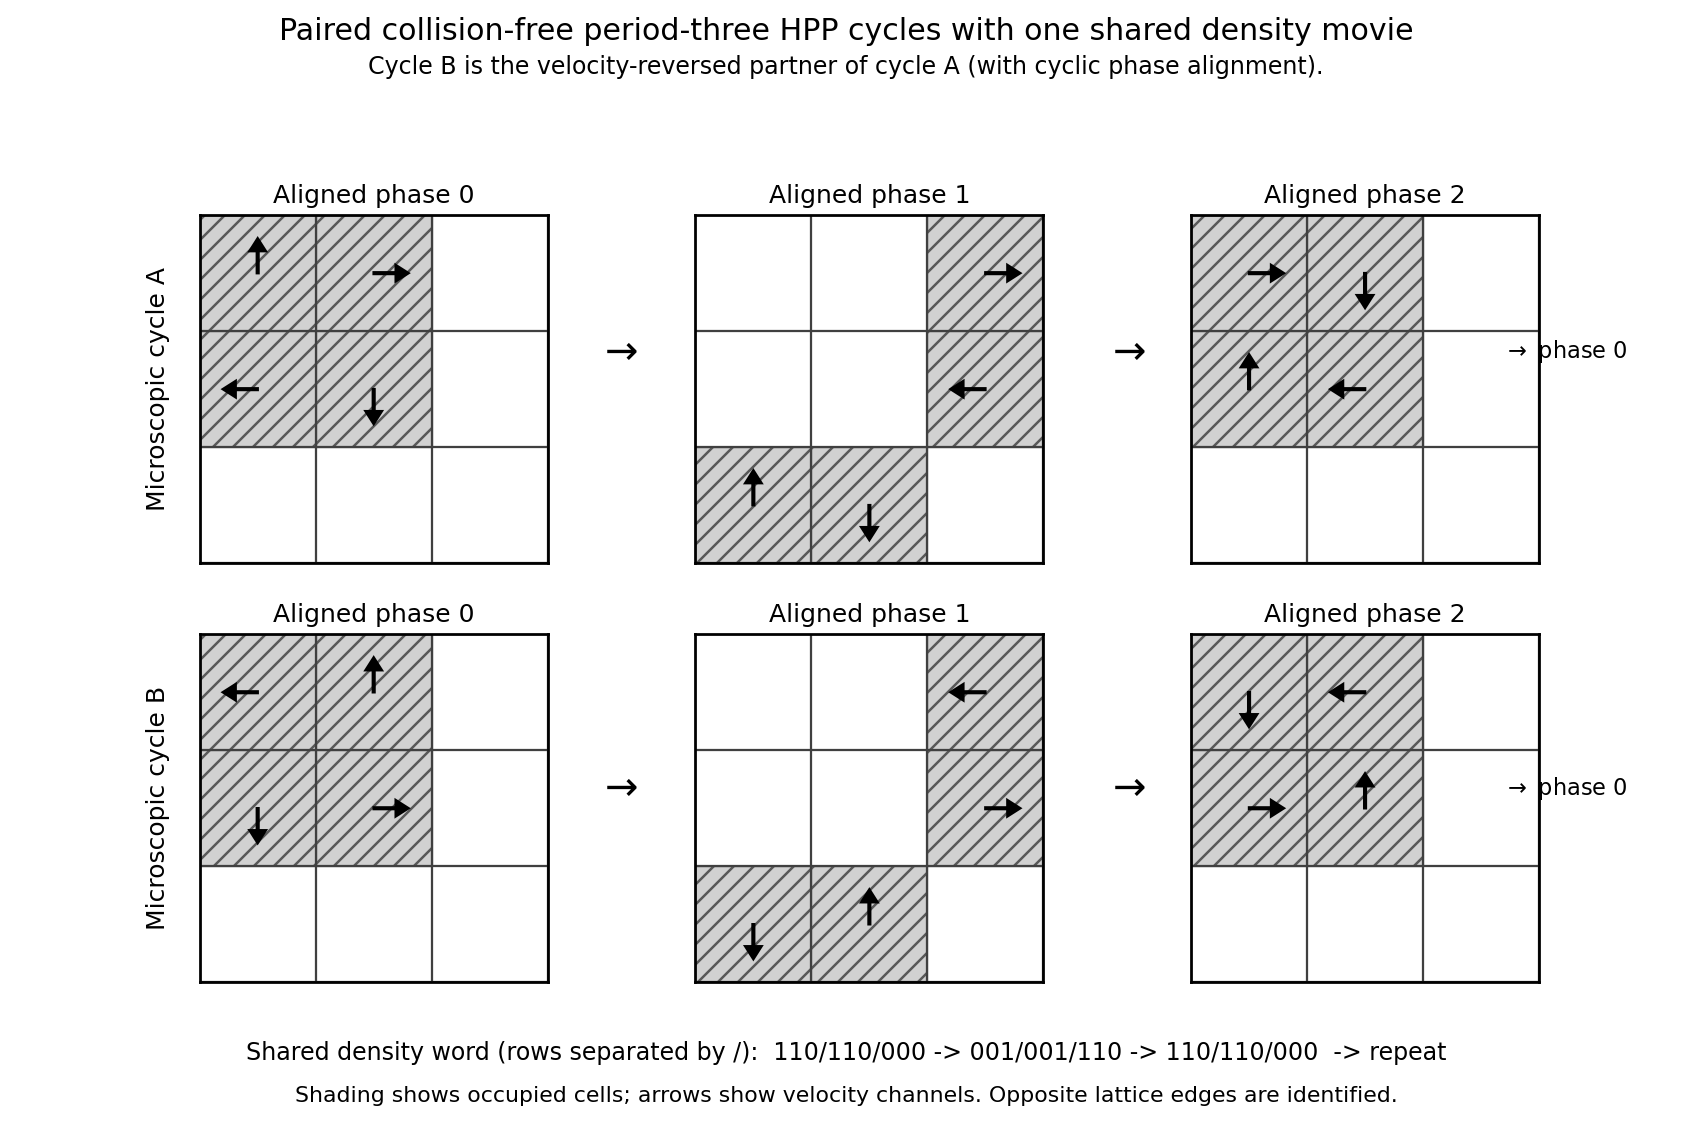
\includegraphics[width=0.98\linewidth]{figures/hpp-ambiguity.png}
  \caption{A self-contained representative of one certified pair on the
  $3\times3$ periodic lattice. The top and bottom rows show the three phases of
  microscopic cycles A and B. Velocity arrows distinguish the complete states;
  identical grayscale occupied-cell shading in each column shows the aligned
  density equality. Cycle B is the velocity-reversed partner of cycle A after the
  indicated phase alignment. Opposite lattice edges are identified, and the
  shared period-three density word is printed beneath the diagrams.}
  \label{fig:hppambiguity}
\end{figure}

Intuitively: ``Density sees where particles are but not which way they are moving.
For these special period-three trajectories, the forward and velocity-reversed
microscopic movies cast the same density shadow forever.'' The statement is
specific to the selected observation and exceptional orbit structure. It is
stronger than equality at one time or over a finite horizon because
\[
h(F^t a_i)=h(F^t b_i)\qquad\text{for every }t\geq0
\]
for each of the 27 aligned phase pairs.

\subsection{Computer-assisted proof and completeness certificate}

The enumeration code discovers the stable predictive partition and writes the
exact catalog. A separate verifier avoids the high-level classification routines:
it reimplements channel collision, streaming, inverse streaming, state encoding,
velocity reversal, and $R=C\circ V$ from low-level definitions. It then reads the
committed exact-data files and independently asserts all of the following:
\begin{itemize}[leftmargin=1.5em]
  \item exactly 9,153 sector states, each satisfying the four-particle and
  zero-momentum constraints;
  \item exactly 9,099 singleton classes and 27 doubletons in the stable predictive
  partition;
  \item exactly 54 distinct cataloged ambiguous states with no omission or
  duplicate assignment;
  \item exactly 18 disjoint cycles, each of least period three and collision-free;
  \item exactly nine involutive time-reversal pairings, with identical density at
  every recorded aligned phase;
  \item correct state, reversed-state, successor, predecessor, density, period,
  phase, pair, and collision fields in every certificate row; and
  \item predictive uniqueness of every nonexceptional state.
\end{itemize}
Assertions terminate with a nonzero status if any item fails. The catalog is thus
a compact machine-checkable certificate, while the theorem explains the symmetry
mechanism behind the certified exceptional set. Enumeration establishes that the
list is complete; time-reversal symmetry explains why its members remain
ambiguous forever.

\subsection{Information-theoretic interpretation}

Using Shannon conditional entropy \cite{shannon1948}, let $X$ now denote a
random microscopic state, uniformly distributed over the 9,153-state sector, let
$W=\Future_h(X)$ be its complete future density sequence, and let $E$ be the
event that $X$ lies in the 54-state exceptional set. Every nonexceptional record
has one compatible microscopic trajectory.
Every exceptional record has exactly two, the two members of one predictive
doubleton. Because the prior weights those two states equally,
\[
H(X\mid W,E)=\log_2 2=1\ \text{bit}.
\]
This is a conditional statement about the exceptional set; density does not
generally lose one bit throughout the sector. Averaging over the uniform sector
prior gives
\[
H(X\mid W)
=\frac{54}{9153}\log_2 2
\approx0.00590\ \text{bits}.
\]
The exceptional fraction is likewise
\[
\frac{54}{9153}\approx0.0058997=0.58997\%.
\]
These values depend on the stated sector, observation map, and prior.

\subsection{Reference orbit and ensemble studies}

A separate specified $5\times5$ HPP microstate has exact period 175. At times 13
and 23 its density fields agree while the velocity microstates differ by eight
bits and their next density fields differ. This demonstrates immediate failure of
one-step density closure on a larger lattice.

Two deterministic paired ensembles test how hidden differences propagate:
\begin{itemize}[leftmargin=1.5em]
  \item In 150 same-sector pairs, particle number, momentum, energy, and the full
  initial density field are identical. All density trajectories separate; 139
  pairs show microscopic Hamming growth; and all 30 resolved cycle audits place
  the pair on different exact cycles.
  \item In 1,200 fixed-channel-filling pairs, all density trajectories separate;
  1,158 show microscopic growth; 20 of 30 capped pair searches close for both
  states, and 19 of those 20 pairs have different periods.
\end{itemize}

\begin{figure}[ht]
  \centering
  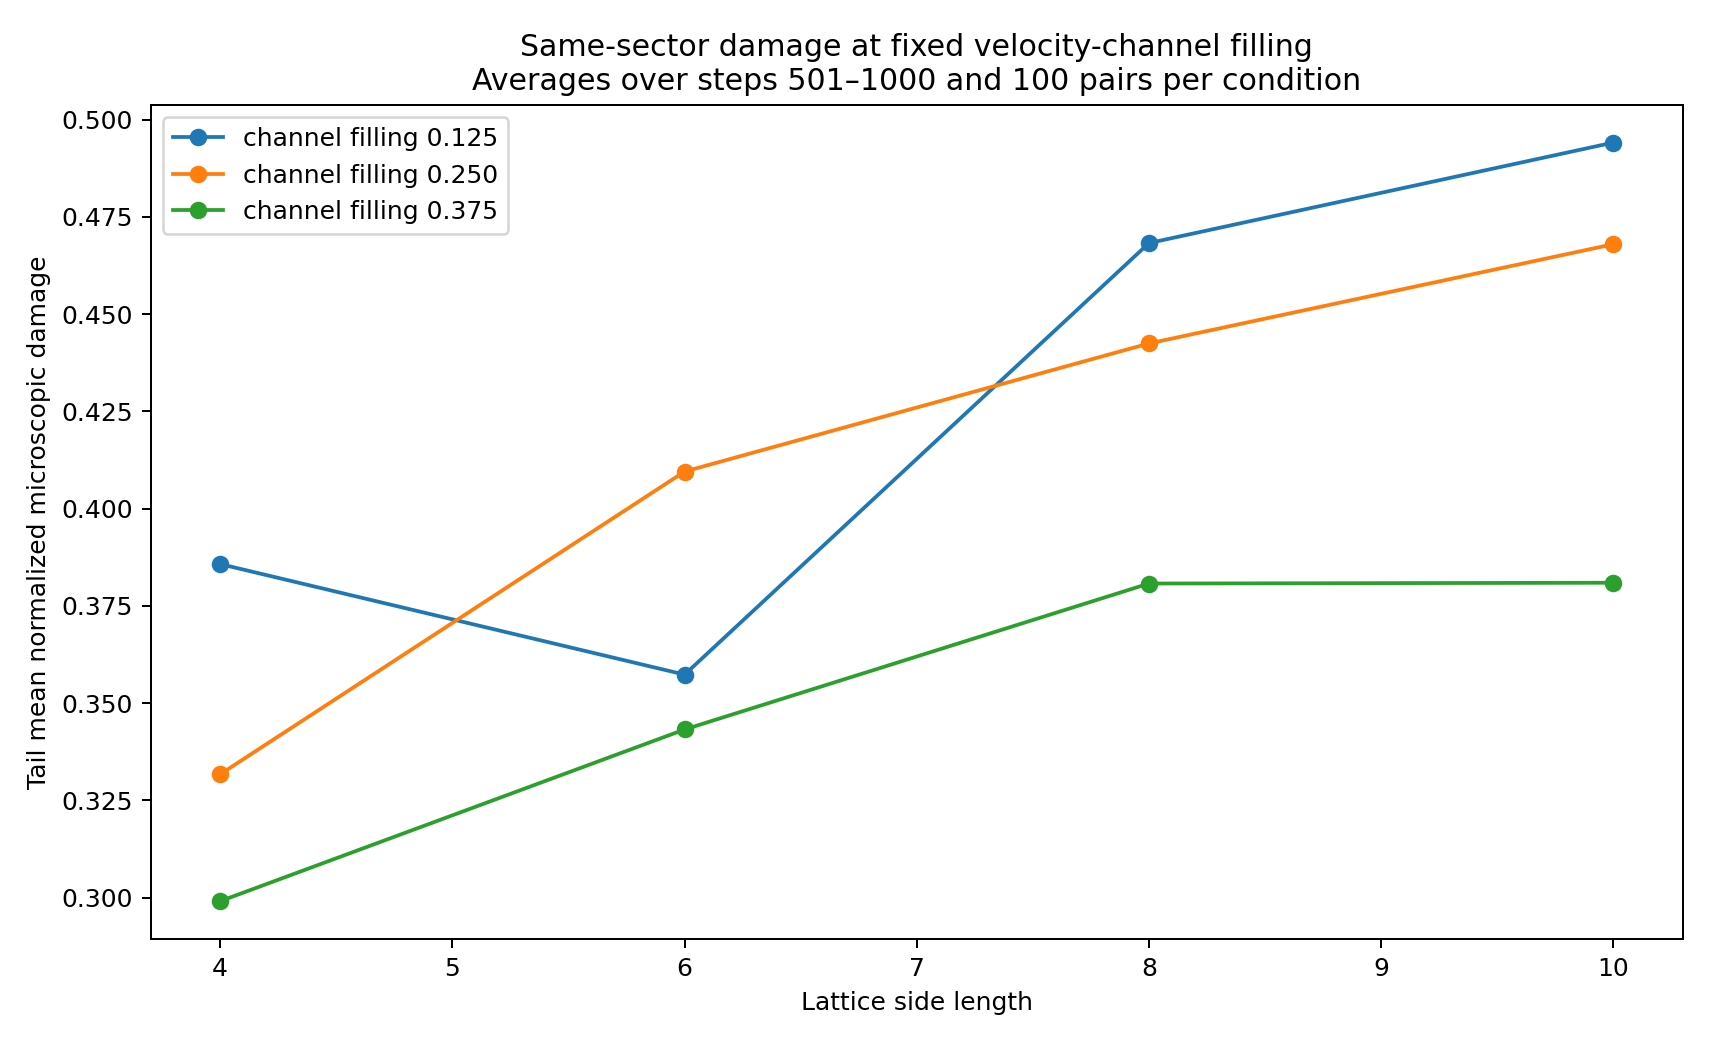
\includegraphics[width=0.76\linewidth]{figures/hpp-damage.png}
  \caption{Mean normalized microscopic Hamming damage in the fixed-density HPP
  ensemble. The curves are finite-time damage diagnostics, not Lyapunov
  exponents. Every trajectory remains periodic because the state space is finite
  and the update is bijective.}
  \label{fig:hppdamage}
\end{figure}

\section{A reversible hexagonal model with hidden collision memory}

The six-direction model uses a local rotor bit to make selected collision rules
exactly reversible. The rotor is part of the complete state even though it is not
part of the particle-density observation. This is a designed reversible model,
not the standard stochastic FHP collision rule of Frisch, Hasslacher, and Pomeau
\cite{frisch1986}.

Across 900 paired trials, every pair begins with identical density, direction
counts, momentum, particle number, and rotor field, but with a four-bit velocity
reassignment. All 900 density trajectories separate. Particle damage grows in
852 pairs and hidden rotor fields separate in 849. The implementation also checks
local collision involution, global inverse evolution, conservation laws, and 300
rotational-covariance trajectories.

\begin{figure}[ht]
  \centering
  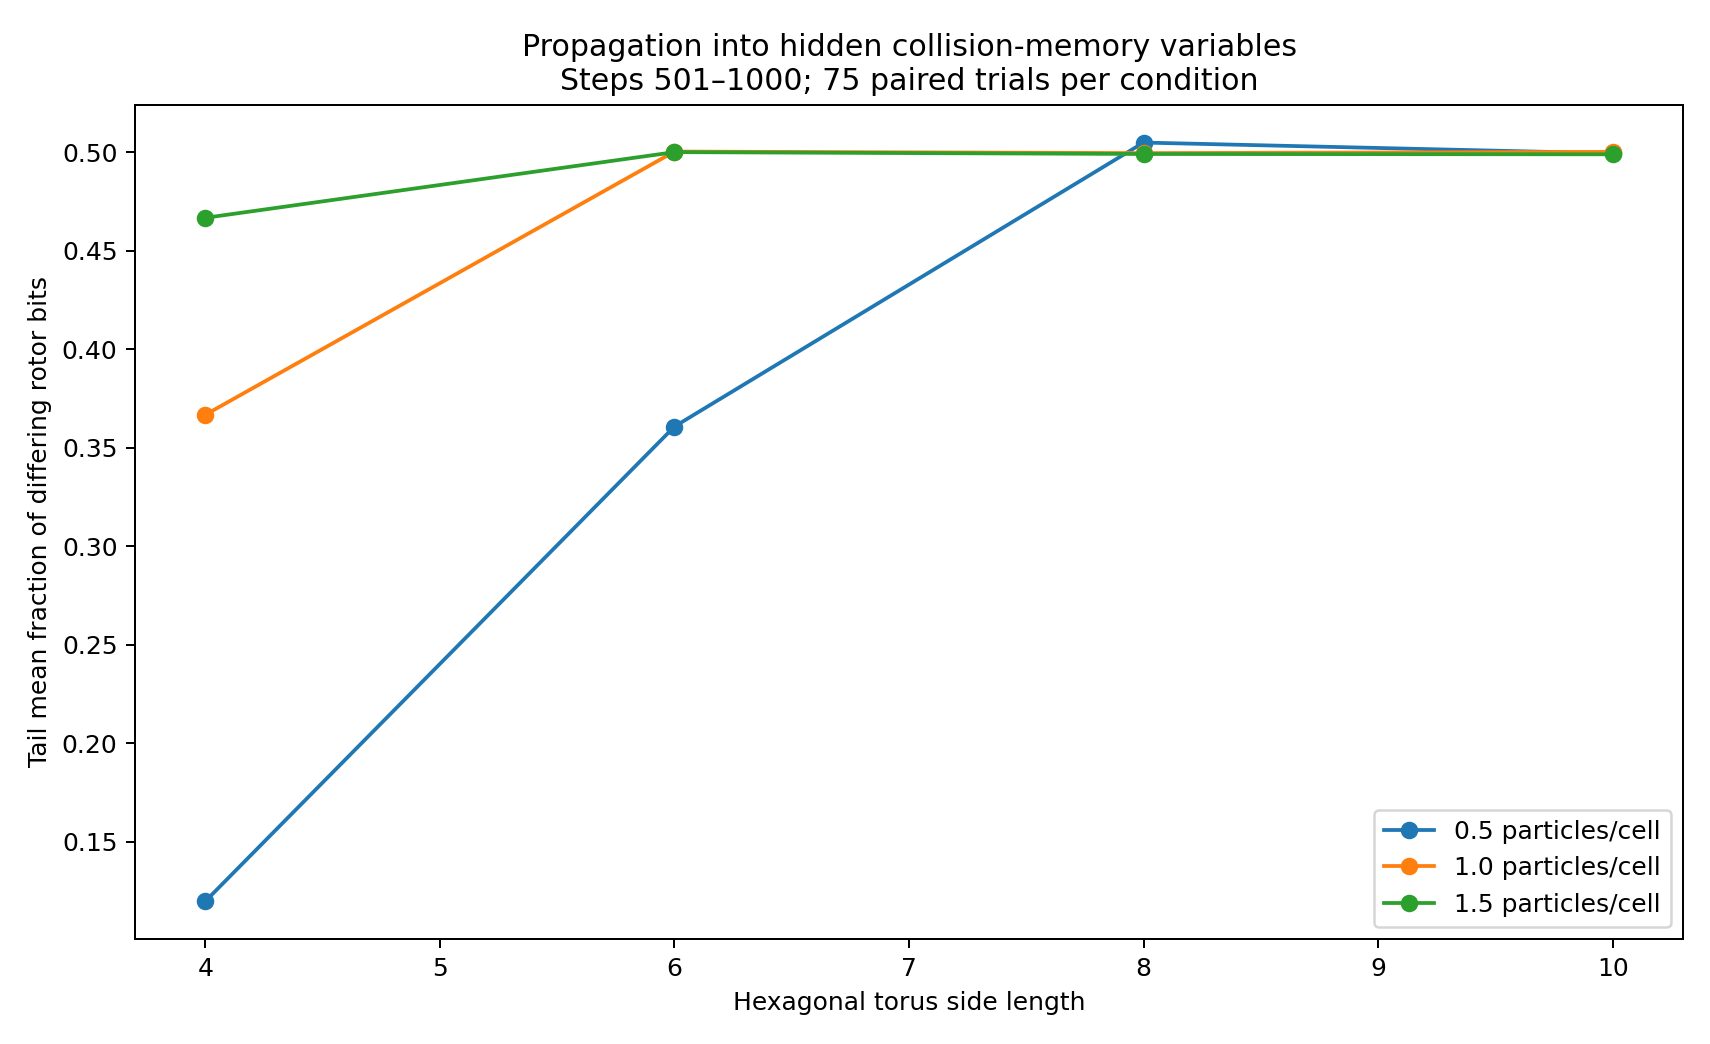
\includegraphics[width=0.76\linewidth]{figures/rotor-damage.png}
  \caption{Propagation of microscopic differences into the hidden rotor field.
  Equality of density and conserved quantities does not fix the collision-memory
  state.}
  \label{fig:rotor}
\end{figure}

\section{Continuous exact and near recurrence}

Finite-state periodicity must be separated from recurrence in continuous phase
spaces.

\subsection{Exact rational hard-particle orbit}

An event-driven ring model uses equal masses, exact rational positions and
velocities, and elastic velocity exchange. The selected labeled complete state
returns after $T=10$ with 36 collision events. Exchanging two initial velocity
labels preserves the position tuple, velocity multiset, total momentum, and
kinetic energy while changing the labeled future. Conserved quantities therefore
do not constitute a complete state.

\begin{figure}[ht]
  \centering
  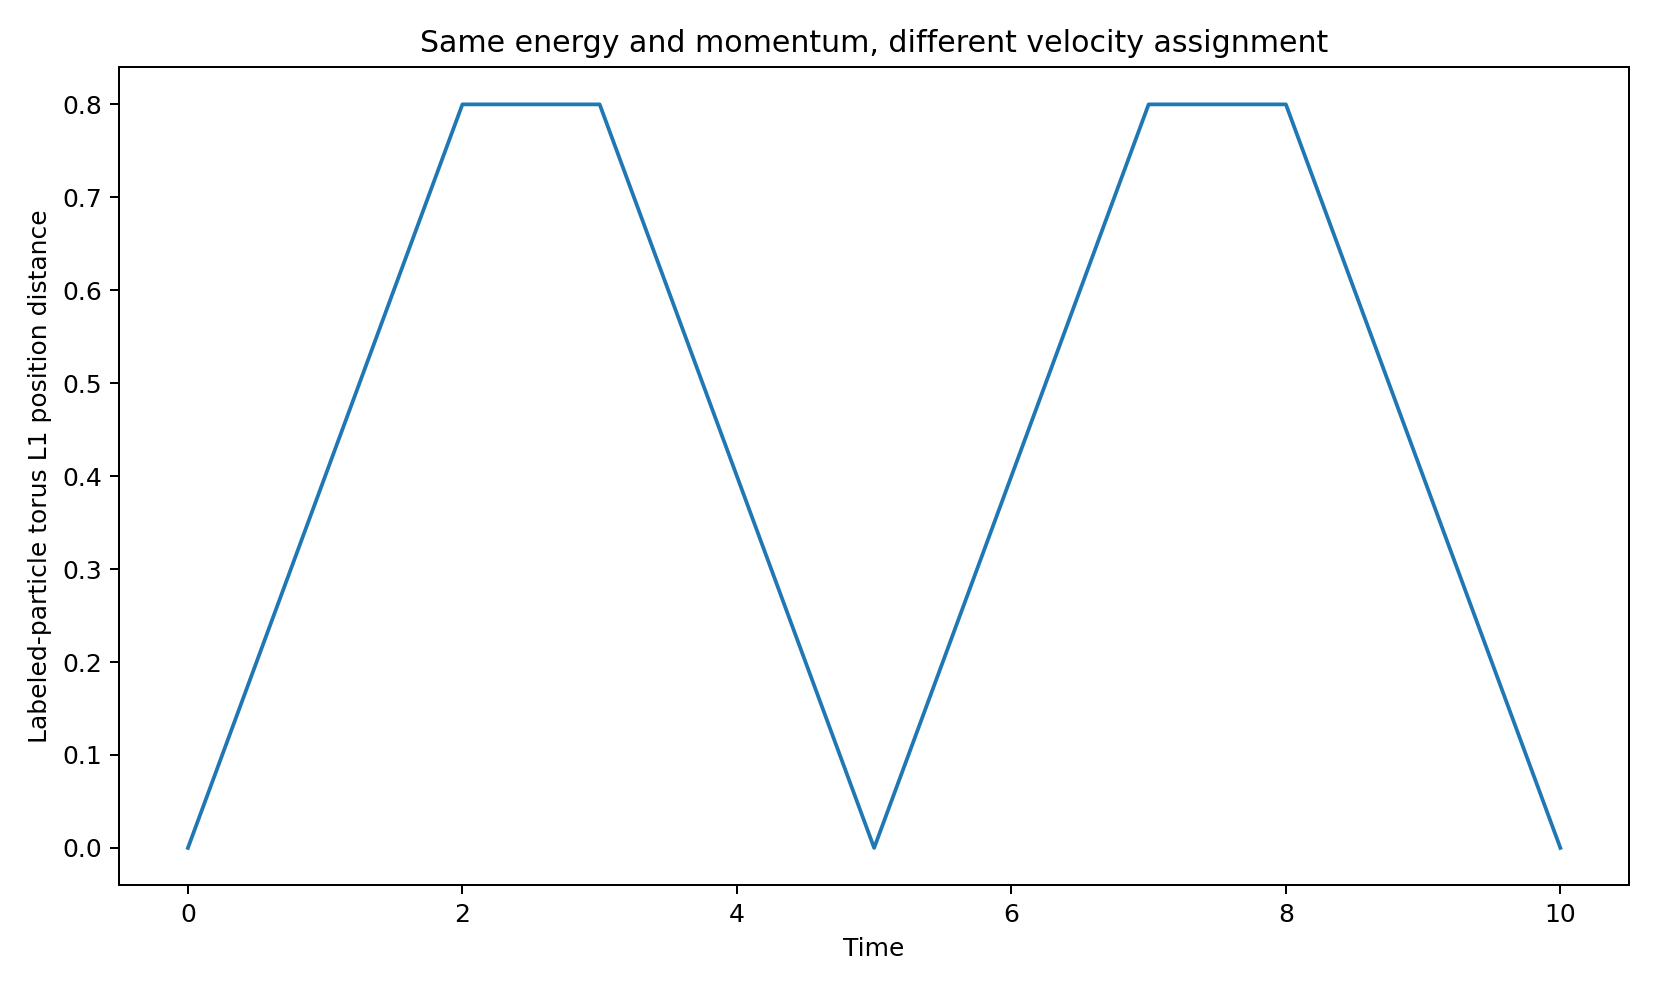
\includegraphics[width=0.76\linewidth]{figures/elastic-distance.png}
  \caption{Exact position-space separation between two labeled hard-particle
  states with the same initial positions, velocity multiset, momentum, and kinetic
  energy.}
  \label{fig:ring}
\end{figure}

\subsection{Irrational torus flow}

Consider
\[
q(t)=(t,\sqrt{2}\,t)\pmod 1.
\]
The flow is deterministic, reversible, compact, and measure preserving. An exact
return at $T>0$ would require both $T\in\Z$ and $\sqrt2T\in\Z$, which would make
$\sqrt2$ rational. No exact positive return exists. Continued-fraction
convergents nevertheless give arbitrarily small return errors, as shown in
\cref{fig:torus}. This is the distinction between exact point recurrence and
Poincar\'e neighborhood recurrence \cite{poincare1890,arnold1989}.

\begin{figure}[ht]
  \centering
  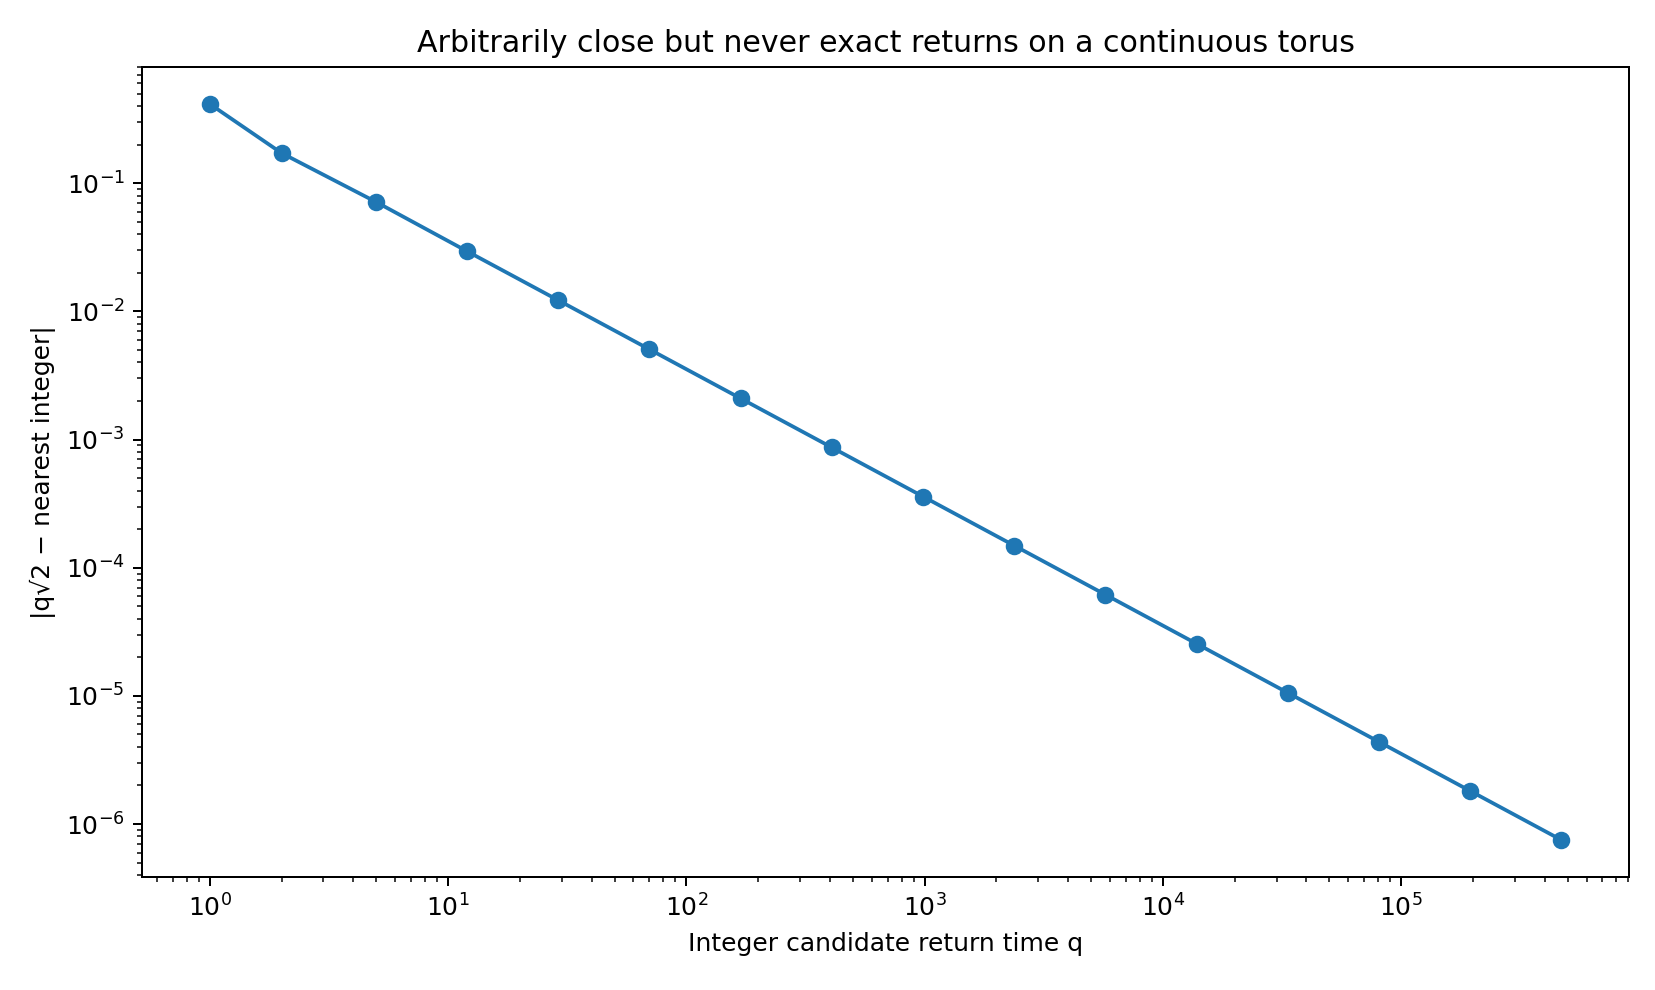
\includegraphics[width=0.76\linewidth]{figures/torus-error.png}
  \caption{Near-return error for convergents to $\sqrt2$. The error decreases but
  never reaches zero.}
  \label{fig:torus}
\end{figure}

\section{Quantum recurrence}

A finite-dimensional Hilbert space is not a finite state set. Normalized vectors,
and the associated projective pure states, form continua. For a time-independent
Hamiltonian,
\[
|\psi(t)\rangle=\sum_n c_n e^{-iE_nt/\hbar}|E_n\rangle.
\]
Physical exact recurrence at time $T$ requires equality up to global phase. Thus
for every pair of occupied levels,
\[
\frac{(E_n-E_m)T}{\hbar}\in2\pi\Z.
\]
Exact recurrence requires commensurate occupied energy gaps. With finitely many
occupied levels, simultaneous phase approximation yields arbitrarily close
returns, which underlies the quantum recurrence theorem
\cite{bocchieri1957,schulman1978}. Continuous spectra, open-system decoherence,
and infinite-dimensional limits require separate treatment.

The finite predictive-partition theorem in this paper does not apply directly to
the continuum of quantum states. Its conceptual lesson still applies: equality
of a reduced measurement record is not automatically equality of the quantum
state, and exact recurrence must be defined at the level of physical states rather
than raw vector phase.

\section{Reproducibility}

The repository distinguishes authoritative source files, deterministic scientific
data, generated figures, and the compiled manuscript. The principal ambiguity
catalog is independently checked rather than trusted because its row count looks
plausible. A clean-reproduction profile regenerates deterministic outputs in a
temporary tree and compares them against the committed data. Scientifically
meaningful figure inputs are checked where binary PDF or rendering details are
not guaranteed to be byte-for-byte stable.

The documented workflow from the repository root is:
\begin{verbatim}
python -m pip install -r requirements.txt -r requirements-dev.txt
python -m pip install -e .
python -m pytest
python scripts/verify_ambiguity.py
python scripts/validate.py reproduction
python scripts/validate.py data
python scripts/validate.py paper
python scripts/validate.py repository
python scripts/validate.py integrity
\end{verbatim}

The `reproduce' profile regenerates committed exact data and figures in place. The
`all' profile runs the tests, independent certificate verifier, clean reproduction,
exact-data assertions, manuscript build, repository hygiene inspection, and
integrity-manifest check. Every script uses repository-relative paths, exits
nonzero on failure, and prints a concise successful result only after its
assertions have passed. Declared cycle-search caps are recorded as censored rather
than treated as evidence of nonrecurrence.

\section{Scope and limitations}

The exact predictive partition is computed for an explicitly finite deterministic
system. The HPP result is exhaustive only for the stated $3\times3$,
four-particle, zero-momentum sector and sitewise-density observation; it is not a
classification of other lattice sizes, particle sectors, collision rules, or
coarse-grainings. The larger-lattice ensembles are finite computational studies
with declared seeds, windows, and cycle caps. The square HPP model is anisotropic.
The rotor model uses a deliberately introduced memory variable. The hard-particle
example is integrable and commensurate by construction.

Moore/Nerode state equivalence, automaton minimization, bisimulation, symbolic
coding, observability, and predictive-state representations supply the established
conceptual setting. The contribution claimed here is the exhaustive HPP
classification, the proof that its permanent ambiguity is exactly nine paired
period-three density movies, the precise time-reversal explanation, and the
reproducible certificate of completeness. No claim is made of peer review,
external replication, novelty priority for the general equivalence construction,
or a universal physical law.

\section{Conclusion}

Repetition of a complete deterministic state fixes the future. Repetition of an
observation does so only when the observation, possibly with a finite history,
identifies the relevant predictive state. Finite partition refinement separates
one-time equality, finite-horizon agreement, exact future equivalence, and
microscopic equality without conflating them.

The HPP classification gives a complete nontrivial failure case. Of 9,153 states,
9,099 are uniquely determined by the full future density record. The remaining 54
states are not arbitrary exceptions: they are 18 collision-free least-period-three
cycles, arranged as nine time-reversal pairs with three aligned phases. The
reversal theorem explains why each pair has the same density future, and the
independent verifier establishes that the catalog exhausts every nonsingleton
predictive class. Under the uniform sector prior, the residual uncertainty is one
bit conditional on the exceptional set and approximately $0.00590$ bits when
averaged over the whole sector.

\begin{thebibliography}{99}
\setlength{\itemsep}{2pt}

\bibitem{moore1956}
E. F. Moore,
``Gedanken-experiments on sequential machines,'' in
\emph{Automata Studies}, Annals of Mathematics Studies Vol. 34,
129--153 (Princeton University Press, 1956).

\bibitem{nerode1958}
A. Nerode,
``Linear automaton transformations,''
\emph{Proceedings of the American Mathematical Society} \textbf{9}, 541--544
(1958).
doi:10.1090/S0002-9939-1958-0135681-9.

\bibitem{park1981}
D. Park,
``Concurrency and automata on infinite sequences,'' in
\emph{Theoretical Computer Science}, Lecture Notes in Computer Science Vol. 104,
167--183 (Springer, 1981).
doi:10.1007/BFb0017309.

\bibitem{sinai1968}
Ya. G. Sinai,
``Markov partitions and C-diffeomorphisms,''
\emph{Functional Analysis and Its Applications} \textbf{2}, 61--82 (1968).
doi:10.1007/BF01075361.

\bibitem{kalman1960}
R. E. Kalman,
``On the general theory of control systems,'' in
\emph{Proceedings of the First International Congress of Automatic Control},
481--492 (Butterworths, 1961).

\bibitem{littman2002}
M. L. Littman, R. S. Sutton, and S. Singh,
``Predictive representations of state,'' in
\emph{Advances in Neural Information Processing Systems 14}, 1555--1561
(MIT Press, 2002).

\bibitem{bennett1973}
C. H. Bennett,
``Logical reversibility of computation,''
\emph{IBM Journal of Research and Development} \textbf{17}, 525--532 (1973).
doi:10.1147/rd.176.0525.

\bibitem{shannon1948}
C. E. Shannon,
``A mathematical theory of communication,''
\emph{Bell System Technical Journal} \textbf{27}, 379--423 and 623--656 (1948).

\bibitem{poincare1890}
H. Poincar\'e,
``Sur le probl\`eme des trois corps et les \'equations de la dynamique,''
\emph{Acta Mathematica} \textbf{13}, 1--270 (1890).
doi:10.1007/BF02392506.

\bibitem{arnold1989}
V. I. Arnold,
\emph{Mathematical Methods of Classical Mechanics}, 2nd ed.
(Springer, 1989).
doi:10.1007/978-1-4757-2063-1.

\bibitem{takens1981}
F. Takens,
``Detecting strange attractors in turbulence,'' in
\emph{Dynamical Systems and Turbulence, Warwick 1980},
Lecture Notes in Mathematics Vol. 898, 366--381 (Springer, 1981).
doi:10.1007/BFb0091924.

\bibitem{sauer1991}
T. Sauer, J. A. Yorke, and M. Casdagli,
``Embedology,''
\emph{Journal of Statistical Physics} \textbf{65}, 579--616 (1991).
doi:10.1007/BF01053745.

\bibitem{paige1987}
R. Paige and R. E. Tarjan,
``Three partition refinement algorithms,''
\emph{SIAM Journal on Computing} \textbf{16}, 973--989 (1987).
doi:10.1137/0216062.

\bibitem{crutchfield1989}
J. P. Crutchfield and K. Young,
``Inferring statistical complexity,''
\emph{Physical Review Letters} \textbf{63}, 105--108 (1989).
doi:10.1103/PhysRevLett.63.105.

\bibitem{hardy1973}
J. Hardy, Y. Pomeau, and O. de Pazzis,
``Time evolution of a two-dimensional model system. I. Invariant states and
time correlation functions,''
\emph{Journal of Mathematical Physics} \textbf{14}, 1746--1759 (1973).
doi:10.1063/1.1666248.

\bibitem{frisch1986}
U. Frisch, B. Hasslacher, and Y. Pomeau,
``Lattice-gas automata for the Navier--Stokes equation,''
\emph{Physical Review Letters} \textbf{56}, 1505--1508 (1986).
doi:10.1103/PhysRevLett.56.1505.

\bibitem{bocchieri1957}
P. Bocchieri and A. Loinger,
``Quantum recurrence theorem,''
\emph{Physical Review} \textbf{107}, 337--338 (1957).
doi:10.1103/PhysRev.107.337.

\bibitem{schulman1978}
L. S. Schulman,
``Note on the quantum recurrence theorem,''
\emph{Physical Review A} \textbf{18}, 2379--2380 (1978).
doi:10.1103/PhysRevA.18.2379.

\end{thebibliography}

\end{document}
